\documentclass[11pt]{article}

\usepackage[utf8]{inputenc}
\usepackage[margin=1in]{geometry}
\usepackage{amsmath, amssymb}
\usepackage{booktabs}
\usepackage{tabularx}
\usepackage{microtype}
\usepackage{titlesec}
\usepackage{xcolor}
\usepackage{listings}
\usepackage{tikz}
\usetikzlibrary{shapes,arrows.meta,positioning,calc}
\usepackage{hyperref}

% --- Color Palette ---
\definecolor{deepink}{HTML}{1A1A2E}
\definecolor{accent}{HTML}{2563EB}
\definecolor{purpleaccent}{HTML}{7C3AED}
\definecolor{codebg}{HTML}{F8F9FA}
\definecolor{codeframe}{HTML}{E2E8F0}
\definecolor{keywordcolor}{HTML}{0891B2}
\definecolor{stringcolor}{HTML}{059669}
\definecolor{commentcolor}{HTML}{64748B}

\hypersetup{
    colorlinks=true,
    linkcolor=accent,
    citecolor=purpleaccent,
    urlcolor=accent
}

\lstset{
    backgroundcolor=\color{codebg},
    basicstyle=\ttfamily\footnotesize,
    breaklines=true,
    captionpos=b,
    commentstyle=\color{commentcolor}\itshape,
    frame=single,
    framerule=0.5pt,
    rulecolor=\color{codeframe},
    keywordstyle=\color{keywordcolor}\bfseries,
    stringstyle=\color{stringcolor},
    showstringspaces=false,
    tabsize=2
}

\titleformat{\section}{\large\bfseries\color{deepink}}{\thesection}{1em}{}
\titleformat{\subsection}{\normalsize\bfseries\color{deepink}}{\thesubsection}{1em}{}

\title{\textbf{Semantic Mechanics: The Cultural Economics of Representation, Pragmatics, and Reclaimed Meaning}}
\author{Anonymous Author(s)}
\date{}

\begin{document}

\maketitle

\begin{abstract}
We introduce \textbf{Semantic Mechanics}, an analytical and economic framework for understanding how symbolic representations emerge, compete, and undergo cultural transformation. Conventional accounts of mathematics and linguistics often treat notations as neutral abstractions and language as a static repository of definitions. In contrast, we model language as a dynamic economic medium governed by transaction costs, signaling games, and value extraction. We investigate two fundamental phenomena: (1) \textit{Representational Genealogy}---how historical notations in calculus and formal syntax were selected not purely by conceptual truth, but by printing ergonomics, institutional capital, and cognitive coordination costs (e.g., Leibniz vs.\ Newton, Chomskyan trees vs.\ Lambek pregroups); and (2) \textit{Semantic Inversion}---the pragmatic mechanism in literature, poetry, and hip-hop vernaculars that reclaims meaning by inverting the polarity of stigmatized signs ($f \mapsto f^{-1}$, e.g., ``bad'', ``ill'', ``sick''). We formulate a dynamical model tracking the lifecycle of semantic assets through minting, in-group liquidity, corporate arbitrage, and semantic inflation, providing an economic lens on cultural evolution and linguistic sovereignty.
\end{abstract}

\section{Introduction: Meaning as Mechanics}

Language is rarely static. It is not an immutable lookup table stored in an institutional dictionary, nor is it merely a passive statistical medium. Language operates as a continuous, dynamical economy: words and notations are minted under social pressure, circulated as credit within trusted groups, targeted for institutional extraction, debased through hyper-inflation, and actively inverted to reclaim autonomy.

Across both elite scientific discourse and grassroots vernacular traditions, the survival and trajectory of a symbol follow strict economic mechanics:
\begin{enumerate}
    \item \textbf{Cognitive and Printing Transaction Costs}: Why did European mathematics adopt $\frac{dy}{dx}$ over $\dot{x}$? Why did linguistics adopt phrase structure trees over string diagrams? The answer lies in the marginal cost of typesetting, pedagogical distribution, and post-war institutional funding.
    \item \textbf{Pragmatic Arbitrage and Sign Inversion}: How do historically marginalized communities resist linguistic subjugation? Through the \textit{semantic inverse}---taking carceral, pathological, or pejorative signifiers and inverting their algebraic valuation to establish in-group sovereignty.
\end{enumerate}

By viewing cultural evolution through the lens of semantic mechanics, we bridge the history of scientific representation with the living poetics of vernacular literature and hip-hop.

\section{The Economic Genealogy of Scientific Notations}

Scientific representations are technologies of coordination. Like physical currencies, notations survive because they minimize friction within specific historical and material infrastructures.

\subsection{The Calculus Wars: Leibniz vs.\ Newton}
The dispute between Gottfried Wilhelm Leibniz and Sir Isaac Newton is celebrated as a priority feud over infinitesimal calculus. Viewed economically, however, it was a battle over \textbf{notational transaction costs}:

\begin{table}[h]
\centering
\small
\begin{tabularx}{\textwidth}{lXX}
\toprule
\textbf{Dimension} & \textbf{Newtonian Fluxions ($\dot{x}, \ddot{x}$)} & \textbf{Leibnizian Differentials ($\frac{dy}{dx}, \int y\,dx$)} \\
\midrule
\textbf{Print Ergonomics} & Expensive: dot accents were fragile, prone to ink-clogging and misprints on movable type. & Cheap: standard horizontal fractions and long-$s$ ligatures easily cast by European foundries. \\
\textbf{Algebraic Composability} & Low: geometric intuition obscured operational rules for higher dimensions and partial derivatives. & High: chain rule manifests algebraically as fraction cancellation ($\frac{dy}{dt} = \frac{dy}{dx} \frac{dx}{dt}$). \\
\textbf{Institutional Velocity} & Restricted to the British Royal Society; isolated by insular academic patronage. & Adopted across continental Europe (Bernoullis, Euler); accelerated student onboarding. \\
\bottomrule
\end{tabularx}
\caption{Comparative economics of Newtonian and Leibnizian representations.}
\label{tab:calculus_war}
\end{table}

Newton's dots were tied to kinematic geometry, requiring the reader to already understand the physical trajectory. Leibniz designed his notation as an algebraic ledger. The European continent outpaced British mathematics for over a century precisely because Leibniz's notation lowered the cognitive barrier to entry and was economically optimized for print reproduction.

\subsection{The Formal Syntax Hegemony: Chomsky vs.\ Lambek}
In mid-20th-century linguistics, a parallel contest occurred between Noam Chomsky's generative phrase structure grammars and Joachim Lambek's categorial calculus:
\begin{itemize}
    \item \textbf{Chomskyan Trees ($S \to NP \; VP$)}: Aligned directly with early digital computing architectures, pushdown automata, and compiler parsing algorithms (Fortran, BNF). Crucially, this work received substantial Cold War military research funding (DARPA, US Air Force, MIT Research Laboratory of Electronics) seeking automated Russian translation.
    \item \textbf{Lambek Pregroups ($a \cdot a^r \to 1$)}: Rooted in non-commutative monoids and adjoint functors. Despite their mathematical elegance and topological symmetry, they lacked the institutional momentum and computing-machine alignment of post-war American computer science.
\end{itemize}

A representation does not dominate because it is uniquely true; it dominates because it is subsidized by institutional capital and hardware constraints.

\section{Semantic Inversion: The Poetics of Reclamation}

If dominant institutions construct representations to codify authority, subcultures invent counter-mechanisms to reclaim agency. In African American Vernacular English (AAVE), African diaspora literature, and hip-hop poetics, this process manifests as the \textbf{Semantic Inverse}.

\begin{figure}[h]
\centering
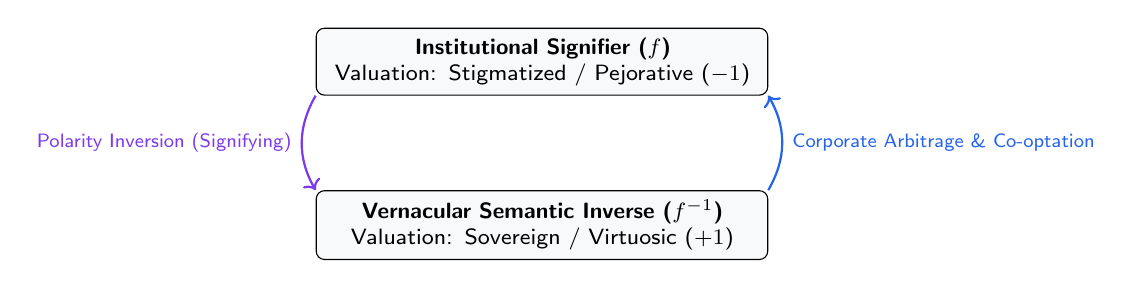
\begin{tikzpicture}[node distance=1.2cm, font=\sffamily\footnotesize]
  \node[draw, rounded corners=3pt, fill=codebg, text width=5.5cm, align=center] (dominant) {
    \textbf{Institutional Signifier ($f$)}\\
    Valuation: Stigmatized / Pejorative ($-1$)
  };
  \node[draw, rounded corners=3pt, fill=codebg, text width=5.5cm, align=center, below=1.2cm of dominant] (reclaimed) {
    \textbf{Vernacular Semantic Inverse ($f^{-1}$)}\\
    Valuation: Sovereign / Virtuosic ($+1$)
  };

  \draw[->, thick, purpleaccent] (dominant.south west) to [bend right=30] node[left, font=\scriptsize\sffamily] {Polarity Inversion (Signifying)} (reclaimed.north west);
  \draw[->, thick, accent] (reclaimed.north east) to [bend right=30] node[right, font=\scriptsize\sffamily] {Corporate Arbitrage \& Co-optation} (dominant.south east);
\end{tikzpicture}
\caption{The dialectical cycle of semantic inversion and institutional arbitrage.}
\label{fig:semantic_cycle}
\end{figure}

\subsection{Polarity Inversion as Cryptographic Agency}
Consider the systematic inversion of adjectives in vernacular traditions:
\begin{itemize}
    \item \textbf{``Bad''} $\mapsto$ Exceptional, formidable, sovereign.
    \item \textbf{``Ill'' / ``Sick''} $\mapsto$ Transcendent skill, virtuosic flow, boundary-breaking execution.
    \item \textbf{``Cold''} $\mapsto$ Unflinching precision, supreme aesthetic detachment.
\end{itemize}

This is not accidental linguistic drift. In Henry Louis Gates Jr.'s formulation of \textit{The Signifying Monkey}, vernacular traditions enact a double-voiced discourse: using the exact lexical tokens of the dominant hierarchy while inverting their pragmatic payload. This inversion operates as a cryptographic defense:
\begin{equation}
    \mathcal{V}(w) = - \mathcal{V}_{\text{inst}}(w)
\end{equation}
An outsider hearing the utterance perceives pathology or condemnation; an insider perceives highest praise. The semantic inverse protects communal credit from immediate institutional surveillance.

\section{The Economic Lifecycle of Linguistic Assets}

Every vernacular token moves through an identifiable lifecycle driven by cultural arbitrage:

\begin{enumerate}
    \item \textbf{Phase 1: Subcultural Minting}. A term is coined under high existential or creative constraint (the street corner, the cipher, the jazz club). It possesses high informational density (Minimum Description Length).
    \item \textbf{Phase 2: In-Group Liquidity}. The term circulates within the community. It functions as high-trust, high-signal social equity.
    \item \textbf{Phase 3: Institutional Arbitrage}. Mainstream advertising agencies, entertainment conglomerates, and social platforms observe the cultural capital. They extract the token to market consumer goods or train models, capturing financial surplus while externalizing the cost to originators.
    \item \textbf{Phase 4: Semantic Debasement \& Inflation}. Once broadcast across mass commercial channels, the token loses its signaling specificity. Its information entropy surges, rendering it sterile (colloquially, ``cringe'').
    \item \textbf{Phase 5: Abandonment \& Re-Minting}. The community abandons the co-opted term and mints a fresh semantic inverse, resetting the cycle.
\end{enumerate}

\section{Computational Simulation}

To evaluate this dynamic, we implemented a discrete-time simulation modeling the interaction between in-group symbolic capital $C(t)$, institutional adoption $A(t)$, and semantic entropy $H(t)$:
\begin{align}
    A(t+1) &= \min\big(1.0, \; A(t) + \alpha \cdot P_{\text{comm}}\big) \\
    C(t+1) &= C(t) \cdot \big(1.0 - \beta \cdot A(t)\big) \\
    H(t+1) &= H(t) + \gamma \cdot A(t)
\end{align}
where $\alpha$ is commercial capture pressure, $\beta$ is the in-group dilution penalty, and $\gamma$ is entropy expansion. When $C(t)$ drops below a threshold and $A(t)$ saturates, the inversion operator triggers:
\begin{equation}
    C_{\text{new}} \leftarrow C_0 \cdot \rho, \quad A_{\text{new}} \leftarrow 0.05, \quad H_{\text{new}} \leftarrow H_0
\end{equation}

Our simulation demonstrates that commercial co-optation inevitably accelerates its own obsolescence: by extracting subcultural tokens to maximize short-term mainstream engagement, institutions destroy the token's distinctiveness, forcing culture to continually innovate at the margins.

\section{Conclusion}

Semantic mechanics reveals that cultural evolution is neither purely random nor purely abstract. Representations in mathematics and linguistics survive because they solve economic coordination problems; vernacular inversions in poetry and hip-hop emerge because communities require resilient mechanisms to preserve symbolic autonomy against commercial extraction. By studying language as a living economic medium, we can better understand both the formal systems of the past and the vernacular innovations shaping the future.

\end{document}
